\frame{
    \frametitle{ $T \bar{T}$ Sample and Track Chains Used in this Presentation } 
    Sample T production of four million events:
    { \small mc16\_13TeV.410470.PhPy8EG\_A14\_ttbar\_hdamp258p75\_nonallhad.
        digit.AOD.e6337\_e5984\_s3126\_r11392\_d1512\_r11391 }

    { \tiny (Based on JIRA Ticket: https://its.cern.ch/jira/browse/ATLMCPROD-7318) }

    \vfill

    \begin{table}
    \resizebox{\textwidth}{!}{%
    \begin{tabular}{| l | l | l | l |}
        \hline
        Trigger Title & Input Chain & Track Key & Prm Vtx Key \\
        \hline \hline
        HLT & HLT\_j35\_boffperf\_split & InDetTrigTrackingxAODCnv\_Bjet\_IDTrig & xPrimVx\\
        FTK IDTrig & HLT\_j35\_boffperf\_split\_FTK\_L1J15 & InDetTrigTrackingxAODCnv\_Bjet\_FTK\_IDTrig & PrimVertexFTK\\
        FTKRefit IDTrig & HLT\_j35\_boffperf\_split\_FTKRefit\_L1J15 & InDetTrigTrackingxAODCnv\_Bjet\_FTKRefit\_IDTrig & PrimVertexFTK\\
        %FTK Refit & HLT\_j35\_boffperf\_split\_FTKRefit\_L1J15\_FTK & InDetTrigTrackingxAODCnv\_Bjet\_FTKRefit & PrimVertexFTK\\
        %FTK-HLT & HLT\_j35\_boffperf\_split\_FTKVtx\_L1J15\_FTK & InDetTrigTrackingxAODCnv\_Bjet\_IDTrig & PrimVertexFTK\\
        \hline
    \end{tabular}}
    \end{table}
}

\frame{
    \begin{figure}
    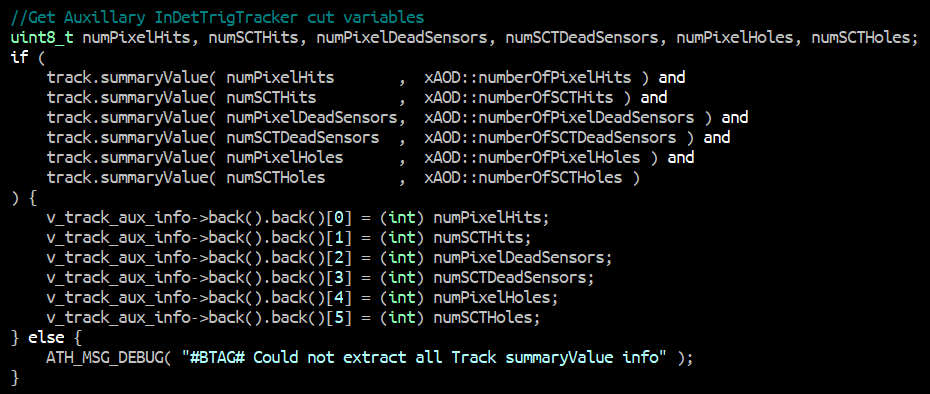
\includegraphics[width=\linewidth,height=\textheight,keepaspectratio]{quality_cut_retrieval}
    \caption{
        \url{https://gitlab.cern.ch/atlas-trigger/b-jet/TrigBtagAnalysis/blob/master/src/BTriggerTuning.cxx\#L1160}
    }
    \end{figure}
}

